%; whizzy chapter
% -initex iniptex -latex platex -format platex -bibtex jbibtex -fmt fmt
% 以上 whizzytex を使用する場合の設定。

%     Kansai Debian Meeting resources
%     Copyright (C) 2007 Takaya Yamashita
%     Thank you for Tokyo Debian Meeting resources

%     This program is free software; you can redistribute it and/or modify
%     it under the terms of the GNU General Public License as published by
%     the Free Software Foundation; either version 2 of the License, or
%     (at your option) any later version.

%     This program is distributed in the hope that it will be useful,
%     but WITHOUT ANY WARRANTY; without even the implied warranty of
%     MERCHANTABILITY or FITNESS FOR A PARTICULAR PURPOSE.  See the
%     GNU General Public License for more details.

%     You should have received a copy of the GNU General Public License
%     along with this program; if not, write to the Free Software
%     Foundation, Inc., 51 Franklin St, Fifth Floor, Boston, MA  02110-1301 USA

%  preview (shell-command (concat "evince " (replace-regexp-in-string "tex$" "pdf"(buffer-file-name)) "&"))
% 画像ファイルを処理するためにはebbを利用してboundingboxを作成。
%(shell-command "cd image200708; ebb *.png")

%%ここからヘッダ開始。

\documentclass[mingoth,a4paper]{jsarticle}
\usepackage{kansaimonthlyreport}
\usepackage[dvips]{xy}

% 日付を定義する、毎月変わります。
\newcommand{\debmtgyear}{2012}
\newcommand{\debmtgdate}{23}
\newcommand{\debmtgmonth}{9}
\newcommand{\debmtgnumber}{64}

\begin{document}

\begin{titlepage}

% 毎月変更する部分、本文の末尾も修正することをわすれずに

 第\debmtgnumber{}回 関西 Debian 勉強会資料

\vspace{2cm}

\begin{center}
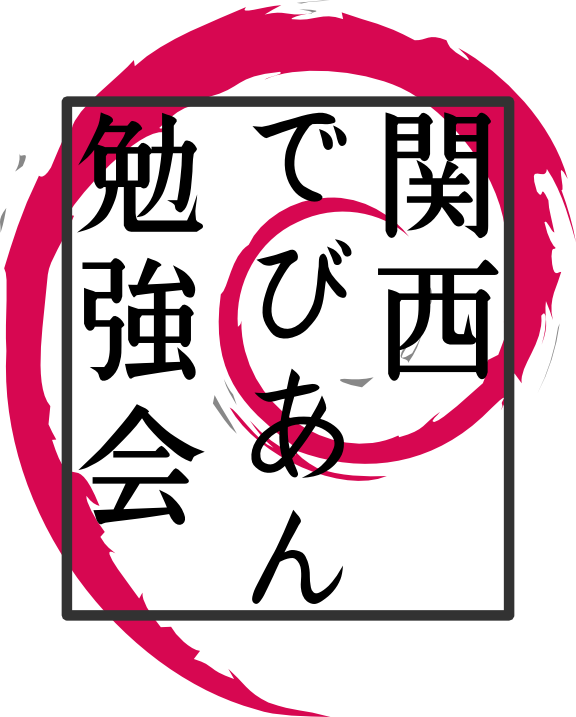
\includegraphics{image200802/kansaidebianlogo.png}
\end{center}

\begin{flushright}
\hfill{}関西 Debian 勉強会担当者 佐々木・倉敷・のがた・かわだ \\
\hfill{}\debmtgyear{}年\debmtgmonth{}月\debmtgdate{}日
\end{flushright}

\thispagestyle{empty}
\end{titlepage}

\dancersection{Introduction}{Debian JP}

 関西Debian勉強会はDebian GNU/Linuxのさまざまなトピック
 (新しいパッケージ、Debian特有の機能の仕組、Debian界隈で起こった出来事、
 などなど)について話し合う会です。

 目的として次の三つを考えています。
 \begin{itemize}
  \item MLや掲示板ではなく、直接顔を合わせる事での情報交換の促進
  \item 定期的に集まれる場所
  \item 資料の作成
 \end{itemize}

 それでは、楽しい一時をお楽しみ下さい。

\newpage

\begin{minipage}[b]{0.2\hsize}
 {\rotatebox{90}{\fontsize{80}{80}
{\gt 関西 Debian 勉強会}}}
\end{minipage}
\begin{minipage}[b]{0.8\hsize}
\hrule
\vspace{2mm}
\hrule
\setcounter{tocdepth}{1}
\tableofcontents
\vspace{2mm}
\hrule
\end{minipage}

\dancersection{最近のDebian関係のイベント報告}{Debian JP}

\subsection{第 63 回関西 Debian 勉強会}

63 回目の関西 Debian 勉強会は 8 月 26 日に福島区民センターで行ないました。

「Debian ではじめる Kerberos 認証」と特別ゲストの Ralf Treinen さんによる「News from EDOS: finding outdated packages」でした。

Ralf さんには DebConf12 のセッションそのままに発表していただきちょっとした DebConf 体験ができたと思います。


\subsection{第 92 回東京エリア Debian 勉強会}
92 回目の東京エリア Debian 勉強会は 9 月 8 日に開催された OSC2012 Tokyo/Fall で行なわれました。

セッションでは「次期安定版 Debian 7.0 "Wheezy" の紹介」を行ない、ブースはインフォグラフィックスやチートシートが好評で多くの方に立ち寄っていただけたようです。
「Grand Unified Debian(あんどきゅめんてっどでびあん 2012夏号)」も完売しました。

\subsection{第 0 回 Debian パッケージング道場 @楽天}
9 月 22 日に楽天にて第 0 回目となる Debian パッケージング道場が開催されました。

丸一日、Debian 漬けで Debian パッケージを作るコアな企画ですが事前申し込み者が 23 名と盛況だったようです。

関西でもこのようなイベントをやりたいですね。


\dancersection{事前課題}{Debian JP}

今回は以下の課題を出題しました.
\begin{screen}
  \begin{enumerate}
  \item Debian を使ってやってみたいことを教えてください。
  \end{enumerate}
\end{screen}

参加者の皆さんの解答は以下の通りです。

\begin{prework}{ 川江 }
  kvmによるWebServer等々の作成
\end{prework}

\begin{prework}{ かわだてつたろう }
  そろそろ開発などを。
\end{prework}

\begin{prework}{ yyatsuo }
  Debian は手段ではなく目的なので特に無し。

  強いて言うならば free の精神を広めること。
\end{prework}

\begin{prework}{ 岡野孝悌 }

翻訳とかしたいですね。

でもって、Debian 関係の翻訳に関する情報をまとめて発表とかしたいですね。

ていうか、かわださんによると近いうちにやることになってますよ \footnote{\url{https://twitter.com/t3rkwd/status/248404019607904256}}。やばい、やばいよ! まずは DDTP に参加だー!
\end{prework}

\begin{prework}{ 木下 }
  \begin{itemize}
  \item 複数のDebianマシンで分散コンパイル

    →できたらいいな的なレベルです\verb!^^;!

    現在AndroidOS開発に携わっているのですが、

    Android2.3以降、ターゲットボードのソースをクリーンビルドすると、

    数時間かかるので、これを複数のDebianマシンで分散コンパイルして

    時間短縮できればいいな的な・・・
  \item DTM等DAW環境として使えたら等・・・
  \item 今更ながらですが、VR等、サイバースペースサーバみたいなシステムとして・・・

    ※この辺、ドシロートです。
  \end{itemize}
\end{prework}

\begin{prework}{ lurdan }
Debian の開発
\end{prework}

\begin{prework}{ 清野陽一 }
自由でオープンな社会の発展
\end{prework}

\begin{prework}{ 山城の国の住人 久保博 }
ソフトウェア開発作業、翻訳作業、Twitter, 年賀状作りなど PC でやる作業全般。そのための環境作りをぼちぼちやって行きたいです。

最近、Xen の準仮想化環境作りに挑戦して、失敗しています。これもやってみたいことの一つです。
\end{prework}

\clearpage

\dancersection{clangによるパッケージビルド}{かわだ てつたろう}

\subsection{はじめに}
「Build of the Debian archive with clang」\cite{clangdebiannet}というDebianのアーカイブをclangで再ビルドするプロジェクトが行なわれています。
clangでパッケージをビルドすることで何がうれしいのかなどを紹介します。

\subsection{clangとは}
clang\footnote{\url{http://clang.llvm.org/}}はC/C++、Objective C/C++を対象としたコンパイラです。
LLVM(Low Level Virtual Machine)\footnote{\url{http://llvm.org/}}をバックエンドとして使用しLLVMの一部としてリリースされています。

clangのサイトに挙げられている機能、目的をいくつかみてみると

\begin{itemize}
\item コンパイルの高速化とメモリ使用低減
\item 親切なメッセージ
\item GCC 互換
\item 高い規格準拠度
\item BSD ライクなライセンス
\item モジュール化されたライブラリ構成
\end{itemize}

といったところがあります。

現在、絶賛開発中なコンパイラです。


\subsection{「Build of the Debian archive with clang」の目標と状況}

プロジェクトの目標は

\begin{itemize}
\item clang が現実的な選択肢であるか(そうでないか)を証明すること
\item 異なるコンパイラを使ってビルドすることによって提供される異なったチェック、警告でソフトウェアのコードの品質を向上すること
\end{itemize}

が挙げられています。

\clearpage

プロジェクトの成果として、2012年6月時点の状況は17710のパッケージが再ビルドされその内2137のパッケージ、全体の12.1\%がビルドに失敗しています。
この結果にはclangを用いたビルドに失敗したがノーマルなsid環境でのビルドに成功したもの、つまりclangのバグと思われるものは含まれていません。

また、過去にはclang2.9、clang3.0を用いてビルドされています。

\begin{table}[h]
  \begin{tabular}{|l|c|r|r|r|} \hline
    clang Ver & 日付 & 対象パッケージ数 & 失敗したパッケージ数 & 失敗したパッケージの割合\\
    \hline \hline
    2.9 & 2011/09 & 16398 & 2372 & 14.5\% \\
    3.0 & 2012/01 & 15658 & 1381 & 8.8\% \\
    3.1 & 2012/06 & 17710 & 2137 & 12.1\% \\
    \hline
  \end{tabular}
\end{table}


\subsection{追試}

プロジェクトのサイトにはビルド環境のセットアップコードが載せられています。
これを用いることで簡単に試してみることができますので試してみましょう。

ただし、セットアップコードを見ていただければ分かりますが/usr/bin\{g++,gcc,cpp\}-VERSIONを一旦削除してclangのシンボリックリンクに置き換えることになります。
常用環境では実行しないほうがよいでしょう。
\\

ここではpbuilderを用いて追試してみました。

pbuilderには環境を変更するための手段としてhookが用意されています。
そこで、先のセットアップコードをhookとして仕込み既存のpbuilder環境を壊すことなく容易にclangビルド環境のセットアップができるようにします。

\begin{commandline}
$ mkdir ~/clanghook
$ cd ~/clanghook
$ cat << EOS > A10replaceclang
#!/bin/sh

echo "Install of clang"
#apt-get update
apt-get install --yes --no-install-recommends clang -t unstable

echo "Replace gcc, g++ & cpp by clang"
VERSION=4.7
cd /usr/bin
rm g++-$VERSION gcc-$VERSION cpp-$VERSION
ln -s clang++ g++-$VERSION
ln -s clang gcc-$VERSION
ln -s clang cpp-$VERSION
cd -

echo "Block the installation of new gcc version"
echo "gcc-4.6 hold"|dpkg --set-selections
echo "cpp-4.6 hold"|dpkg --set-selections
echo "g++-4.6 hold"|dpkg --set-selections
echo "gcc-4.7 hold"|dpkg --set-selections
echo "cpp-4.7 hold"|dpkg --set-selections
echo "g++-4.7 hold"|dpkg --set-selections

echo "Check if gcc, g++ & cpp are actually clang"
gcc --version|grep clang > /dev/null || exit 1
EOS
$ chmod +x A10replaceclang
$ ln -s A10replaceclang F10replaceclang
\end{commandline}
%$

シンボリックリンクを作成することでloginまたはexecute時にもセットアップされるようにしておきます。
\\

これで準備が整いましたので後はpbuilderでパッケージをビルドする時にhookを指定すればclangを使ってビルドされるようになります。

\begin{commandline}
$ sudo pbuilder --build --hookdir ~/clanghook hello_2.8-2.dsc
\end{commandline}
%$

いくつかのパッケージを試してみましたが確かにclangを用いたビルドの方がエラーチェックが厳しいようです。
しかしgccで出力されていた警告がclangでは出力されなくなるケース\footnote{例えば sl\_3.03-17}もありました。
この辺りはコンパイラへのオプションによって変わってくるのかもしれません。


\subsection{libc++}

libc++はclangと同じLLVMのプロジェクトでC++11をターゲットにしたC++標準ライブラリです。
新しい仕様であるC++11への対応はclangのみではなく標準ライブラリの対応も必要で、clangによるC++11への対応といった場合はlibc++を用いた場合かlibstdc++へパッチを当てたものになるようです。
\cite{clang11support}
\\

このlibc++を使うことはプロジェクト展望に「libc++をlibstdc++の代替として提供する」\cite{altlibc++}として含まれています。
この試みは順調に進んでおり、2012/07/31にはlibc++がexperimentalに入りました。まだlibc++自体に問題が多いようですがそれなりに使えています。
\\

パッケージはi386とamd64版しか用意されていませんが、試してみようと思われる方はapt-lineにexperimentalを追加しlibc++-devとlibc++abi-devをインストールしてください。

\begin{commandline}
$ sudo apt-get -t experimental libc++-dev libc++abi-dev
\end{commandline}
%$

そして、適当にC++のコードを書いて、コンパイラへオプションで標準ライブラリにlibc++を指定してビルドします。
出来上がった実行ファイルをlddで表示してみるとlibstdc++ではなくlibc++がリンクされていることが確認できます。
\cite{newc++stdlibindebian}

\begin{commandline}
$ clang++ -stdlib=libc++ foo.cpp -o foo
$ ldd foo|grep c\\+\\+
ldd foo|grep c\\+\\+
  libc++.so.1 => /usr/lib/x86_64-linux-gnu/libc++.so.1 (0x00007f8b5ec60000)
\end{commandline}

\begin{commandline}
$ g++ -nostdlib -lc++ -lc++abi -std=c++11 \
  /usr/lib/x86_64-linux-gnu/crt1.o \
  /usr/lib/x86_64-linux-gnu/crti.o \
  /usr/lib/x86_64-linux-gnu/crtn.o \
  -isystem /usr/include/c++/v1 -lc -lgcc_s \
  foo.cpp -o foo
$ ldd foo|grep c\\+\\+
ldd foo|grep c\\+\\+
  libc++.so.1 => /usr/lib/x86_64-linux-gnu/libc++.so.1 (0x00007f5098ce8000)
  libc++abi.so.1 => /usr/lib/x86_64-linux-gnu/libc++abi.so.1 (0x00007f5098a9a000)
\end{commandline}

さらにC++11の機能を使ってやってみようと思う方は8月の東京エリアDebian勉強会の資料を参考にして試してみてください。

\begin{thebibliography}{9}

\bibitem{clangdebiannet}
Build of the Debian archive with clang, \url{http://clang.debian.net/}

\bibitem{clang11support} 
C++98 and C++11 Support in Clang, \url{http://clang.llvm.org/cxx_status.html}

\bibitem{altlibc++}
Provide an alternative to libstdc++ with libc++, \url{http://wiki.debian.org/SummerOfCode2012/Projects\#Provide_an_alternative_to_libstdc.2B-.2B-_with_libc.2B-.2B-}

\bibitem{newc++stdlibindebian}
Article complet: libc++: New C++ standard library in Debian, \url{http://sylvestre.ledru.info/blog/sylvestre/2012/08/15/libc_new_c_standard_library_in_debian}

\end{thebibliography}

\clearpage

\dancersection{月刊 Debian Policy 第6回 「文書」}{岡野孝悌}

Debian ユーザーでもないのに今回の担当となりました おかの です。

今回読むのは第12章の「文書」についてです。
多くのソフトウェアパッケージにはマニュアルなどの文書が附属していますし、文書のみからなるパッケージもあります (debian-policy 自体がまさにそうです)。
また、マニュアル類のほか、設定ファイルのサンプルや、変更履歴、著作権情報といったものもあります。

\subsection{マニュアル (man ページ)}
ベル研で Unix が誕生したころ、文書処理システムという口実で予算を取っていたりして、
Unix 関係の文書といえば roff でした\footnote{History of UNIX Manpages http://manpages.bsd.lv/history.html が参考になります。}。
本章でも man ページの説明に多くを割いています。

\subsubsection{インストール場所}
roff ファイルを gzip -9 で圧縮して、
{\tt /usr/share/man} 以下の適切な場所にインストールします。
英語マニュアルは {\tt /usr/share/man} 直下、
それ以外は {\tt /usr/share/man/}{\it locale} 以下の、
セクション別のディレクトリ ({\tt man1}, {\tt man2}, ..., {\tt man9}) に置きます。
詳細は FHS 参照といいつつ、FHS とは以下のような差異があります。

\begin{itemize}
\item 英語マニュアルは {\tt /usr/share/man/en} 以下ではなく {\tt /usr/share/man} 直下に置く。
(FHS でこれが許されるのは、英語マニュアルしかない場合)
\item セクション 9 が存在する
(FHS では 1 から 8 までのみ)
\end{itemize}

man ページの整形には時間がかかるので、
整形済みのマニュアルをあらかじめインストールしておけば\footnote{FreeBSD のベースシステムなどでは整形済みのマニュアルが標準で配布されています。}、
いきなりページャーで表示することができて快適になりますが、
パッケージが整形済みマニュアルをインストールしてはいけません。

\subsubsection{パッケージへの同梱}
man ページ以外の文書は、{\it foo}-doc のようにソフトウェア本体と別パッケージに分離することがありますが、
man ページはソフトウェア本体と同じパッケージに含めるのが原則です。

プログラムのマニュアルが存在しない場合、それはバグとして扱われます。
上流にマニュアルを追加してもらうか、Debian パッケージで独自にマニュアルを追加する必要があります。
といっても、「info 見れ」「この URL 見れ」だけのマニュアル\footnote{そのようなマニュアルの実例としては、(いずれも上流由来ですが) GNU cpio や netpbm があります。}でも可です。

\subsubsection{複数名をもつマニュアル}

grep, fgrep, egrep のように、同じマニュアルが複数の名前で参照されることがあります。

Linux Man Page Howto\footnote{\url{ http://www.schweikhardt.net/man_page_howto.html} (JF に古い日本語訳あり)}
では、(シンボリックリンクを持たないシステムに配慮し) roff の .so マクロを使う方法がもっとも望ましいとされていますが、
Debian では必ずシンボリックリンクがあるためか、原則として .so マクロを使わずにシンボリックリンクを使うよう求めています。
ただし、上流で .so マクロを使っている場合は、無理にシンボリックリンクに直す必要はありません。

たとえば grep パッケージ (GNU grep) では、egrep.1.gz, fgrep.1.gz はいずれも grep.1.gz へのシンボリックリンクとなっています。
いっぽう、manpages-ja パッケージにはこれらの (古い) 日本語訳がありますが、こちらでは egrep.1 や fgrep.1 は .so マクロを使って grep.1 を参照しています。

なお、これとは逆に、複数の異なるマニュアルが同じ名前で参照されることがあります。たとえば vim と nvi は、通常どちらも vi という名前で参照されます。
本章では言及されていませんが、これは Appendix F で説明されている update-alternatives で扱うことができます。
また、editor(1) と pager(1) について11章で言及されています。

\subsubsection{翻訳マニュアル}

マニュアル以外の文書にも翻訳はありますが、debian-policy ではマニュアルについてのみ翻訳に触れています。
マニュアルはガンガン更新されるので、せっかく翻訳してもすぐ古くなってしまいます。
利用者が古い翻訳マニュアルを鵜呑みにしないように、翻訳が古い可能性について言及したりするよう求めています。

apt など、Debian 独自ツールのマニュアル翻訳では、po4a を使って翻訳し (訳が古くなった場合、その部分は原文が表示されるようになる)、
かつ注意書きをすることで、この指針が守られているようです。
一方、manpages-ja をはじめ、上流で翻訳されたマニュアルでは、守られていないように見えます。

エンコーディングは UTF-8 のほか、一部のレガシーエンコーディング (日本語の場合は EUC-JP) も使えます\footnote{man のエンコーディングに関する議論は Bug\#440420 参照}。

\subsection{info 文書}

info 文書について述べています。info 文書は必須ではありません。

\begin{itemize}
\item info 文書は {\tt /usr/share/info} 以下へインストールする
\item gzip -9 で圧縮する
\item install-info 用のセクションとディレクトリエントリ情報を含める
\end{itemize}

\subsection{追加文書}

man, info 以外の形式の文書がパッケージに含まれている場合の扱いを述べています。

\begin{itemize}
\item info は {\tt /usr/share/doc/}{\it package} 以下へインストールする
\item 大容量で必要性の低い文書は別パッケージにするべき
\item ソフトウェアの動作が {\tt /usr/share/doc/}{\it package} 以下のファイルに依存してはいけない
\item {\tt /usr/share/doc/}{\it package} 自体を他へのシンボリックリンクとできる条件 (著作権関連情報の節にも記載がありますが、適切な copyright ファイルを機械的に抽出できる必要があります)
\item {\tt /usr/doc} から {\tt /usr/share/doc} への移行に関する説明\footnote{脚注にも説明がありますが、
FSSTND 1.2 までは、{\tt man} や {\tt doc} 等は{\tt /usr/} 直下に置くこととなっていました。
FHS 2.0 (1997 年) で、BSD の流儀を取り入れ、{\tt /usr/share/} 以下に置くよう改められています。
Debian では potato で移行しています。当時の議論は 1999 年からの debian-ctte メーリングリストのログで見ることができます。}
\end{itemize}

\subsection{好ましい文書形式}

DocBook などをもとに同じ文書を複数形式で提供するケースがありますが、
そのような場合は可能な限り HTML をインストールします。
HTML 以外の形式をどうするかはメンテナーの裁量にまかされています。

\subsection{著作権関連情報}

パッケージに含まれるものの著作権、ライセンスに関する文書 ({\tt copyright} ファイル) の扱いについて述べています。このファイルは必須です。

Debian パッケージでは {\tt debian/copyright} に含めておき、
{\tt /usr/share/doc/}{\it package}{\tt /copyright} にインストールします。

このファイルには、パッケージの著作権、ライセンス情報を、元のままで含める必要があります
(ただし、GPL などのよく使われるライセンスは {\tt /usr/share/common-licenses} にあらかじめ置かれているものを参照する形にします)。
内容の改変はもとより、文書形式の変換もしてはいけません。
また、このファイルを圧縮したりシンボリックリンクにしたりしてはいけません。

{\tt copyright} ファイルには、著作権、ライセンス情報のほか、以下の情報を含める必要があります。

\begin{itemize}
\item 上流のソースの入手元
\item パッケージの原作者名
\end{itemize}

また、以下の情報を含めるべきです。

\begin{itemize}
\item Debian パッケージ作成に関与した Debian メンテナ名 (3.9.3.0 で削除されました; 後述)
\item (contrib, non-free の場合) 当該パッケージが Debian の一部ではないことと、その簡潔な理由
\end{itemize}

\subsection{設定例など}

設定ファイルやソースファイルなどの例を提供する場合の扱いを述べています。

\begin{itemize}
\item {\tt /usr/share/doc/}{\it package}{\tt /examples} 以下にインストールする。
\item ただし、アーキテクチャー依存のファイルは
{\tt /usr/lib/}{\it package}{\tt /examples} 以下にインストールし、
シンボリックリンクを張る。
\item 前述のとおり、動作が {\tt /usr/share/doc} 以下のファイルに依存してはいけないので、
ここに置かれたファイルをプログラムから参照してはいけない。
\item {\it foo}-examples のような、例そのものを提供するパッケージは、
パッケージそのものを {\tt /usr/share/doc/}{\it package} にインストールしてもよい。
\end{itemize}

\subsection{Changelog ファイル}

変更履歴の扱いについて述べています。

Debian 由来でないパッケージは、上流の変更履歴と Debian パッケージの変更履歴を区別することを求めています。

\begin{itemize}
\item Debian ソースツリー内の
{\tt debian/changelog} の圧縮されたコピーを
{\tt /usr/share/doc/}{\it package}/{\tt changelog.Debian.gz} としてアクセスできるようにしなければならない。
\item 上流の changelog がある場合は、プレインテキスト形式で、
{\tt /usr/share/doc/}{\it package}{\tt /changelog.gz} としてアクセスできるようにすべき。
\item changelog ファイルが HTML 形式の場合は、
{\tt /usr/share/doc/}{\it package}{\tt /changelog.html.gz} で参照できるようにすべき。
\item 上流のファイル形式の違いによって、別のファイル名を参照しないといけないなどというのはウンコなので、
Lynx を使って HTML をプレインテキストに変換したものを {\tt /changelog.gz} で提供すべき。
\item gzip -9 で圧縮すべき
\end{itemize}

\subsection{最近の変更点}
日本語訳版がある Version 3.9.1.0 から Version 3.9.4.0 までに加えられた変更点を押さえておきましょう。

\subsubsection{Version 3.9.2.0}
\begin{itemize}
\item 「Debian GNU/Linux ディストリビューション」が「Debian ディストリビューション」と改められました。(Bug\#594656)
\item debmake で生成される man のサンプルについて言及されていましたが、lenny 以降では debmake は削除されているため、この記述が削除されました。
\end{itemize}

\subsubsection{Version 3.9.3.0}
\begin{itemize}
\item {\tt copyright} ファイルに Debian パッケージのメンテナーを記述することとされていましたが、{\tt changelog} ファイルに書かれているものなので、{\tt copyright} ファイルへの記述がなくなりました。(Bug\#593533)
\end{itemize}

\vspace{1ex}
\hrule
\subsubsubsection{Version 3.9.2.0 policy.sgml:9771}\par
\parbox{0.48\linewidth}{
	  In addition, the copyright file must say where the upstream
	  sources (if any) were obtained.  It should name the original
	  authors of the package and the Debian maintainer(s) who were
	  involved with its creation.
}\hfil 
\parbox{0.48\linewidth}{
	  また、著作権情報ファイル中には元となった上流のソースをどこから手に入れたかを記載しなければなりません。
	  またパッケージの原作者の名前とパッケージ作成に関与した
	  Debian メンテナの名前を載せるべきです。
}
\hrule

\subsubsubsection{Version 3.9.3.0 policy.sgml:9863}\par
\parbox{0.48\linewidth}{
	  In addition, the copyright file must say where the upstream
	  sources (if any) were obtained, and should name the original
	  authors.
}\hfil 
\parbox{0.48\linewidth}{
	  また、著作権情報ファイル中には元となった上流のソースをどこから手に入れたかを記載しなければなりませんし、
	  パッケージの原作者の名前を載せるべきです。
}
\hrule
\vspace{1ex}

\clearpage

\begin{itemize}
\item 「機械的に抽出」できるようにするもの ({\tt copyright} ファイル) が何を指しているかが、明確に記述されるようになりました。(Bug\#617516)
\end{itemize}

\vspace{1ex}
\hrule
\subsubsubsection{Version 3.9.2.0 policy.sgml:9704}\par
\parbox{0.48\linewidth}{
	  {\tt /usr/share/doc/}{\it package} may be a symbolic
	  link to another directory in {\tt /usr/share/doc} only if
	  the two packages both come from the same source and the
	  first package Depends on the second.  These rules are
	  important because copyrights must be extractable by
	  mechanical means.
}\hfil 
\parbox{0.48\linewidth}{
	  {\tt/usr/share/doc/}{\it package}
	  は、{\tt /usr/share/doc}
	  以下の他のディレクトリ中のシンボリックリンクの相手先と同じソースファイルから作成されたものであること、および相手先に対して
	  "Depends" で依存していることが宣言されていること、の二つの条件を満たすときのみ、シンボリックリンクとすることができます。
	  この規則は、著作権関連ファイルが機械的に抽出できるようにするために大切になるものです。
}
\hrule

\subsubsubsection{Version 3.9.3.0 policy.sgml:9796}\par
\parbox{0.48\linewidth}{
	  {\tt /usr/share/doc/}{\it package} may be a symbolic
	  link to another directory in {\tt /usr/share/doc} only if
	  the two packages both come from the same source and the
	  first package Depends on the second.  These rules are important
	  because {\tt copyright} files must be extractable by
	  mechanical means.
}\hfil 
\parbox{0.48\linewidth}{
	  {\tt/usr/share/doc/}{\it package}
	  は、{\tt /usr/share/doc}
	  以下の他のディレクトリ中のシンボリックリンクの相手先と同じソースファイルから作成されたものであること、および相手先に対して
	  "Depends" で依存していることが宣言されていること、の二つの条件を満たすときのみ、シンボリックリンクとすることができます。
	  この規則は、{\tt copyright} ファイルが機械的に抽出できるようにするために大切になるものです。
}
\hrule
\vspace{1ex}

\begin{itemize}
\item 機械可読な著作権情報ファイルに関する記述が追加されました。ライセンス衝突などの問題を自動的にチェックしたりできることが期待できますが、今のところはオプション扱いです。
\end{itemize}

\vspace{1ex}
\hrule
\subsubsubsection{Version 3.9.3.0 policy.sgml:9928}\par
\parbox{0.48\linewidth}{
	  {\bf Machine-readable copyright information}

	    A specification for a standard, machine-readable format
	    for {\tt debian/copyright} files is maintained as part
	    of the {\it debian-policy} package.  This
	    document may be found in the {\tt copyright-format}
	    files in the {\it debian-policy} package.  It is
	    also available from the Debian web mirrors at
		     \url{http://www.debian.org/doc/packaging-manuals/copyright-format/1.0/}.

	    Use of this format is optional.
}\hfil 
\parbox{0.48\linewidth}{
	  {\bf 機械可読な著作権情報}

	    標準のための仕様として、機械可読な形式の
	    {\tt debian/copyright} ファイルが、
	    この {\it debian-policy} パッケージの一部として保守されています。
	    この文書は {\it debian-policy} パッケージに
	    {\tt copyright-format} ファイルとして含まれています。
	    また、Debian web ミラーの
		     \url{http://www.debian.org/doc/packaging-manuals/copyright-format/1.0/} にもあります。

	    この形式を使うかどうかは任意です。
}
\hrule
\vspace{1ex}

\clearpage

\subsubsection{Version 3.9.3.1}

(変更なし)

\subsubsection{Version 3.9.4.0}
\begin{itemize}
\item {\tt copyright} ファイルのエンコーディングに関する一文が追加されました。(Bug\#661933)
\end{itemize}

\vspace{1ex}
\hrule
\subsubsubsection{Version 3.9.1.0 policy.sgml:10673}\par
\parbox{0.48\linewidth}{
	  All copyright files must be encoded in UTF-8.
}\hfil 
\parbox{0.48\linewidth}{
	  copyright ファイルはすべて UTF-8 でエンコードしなければなりません。
}
\hrule
\vspace{1ex}

\subsection{最後に}
次回の月刊 Debian Policy は。。。

\clearpage

\dancersection{今後の予定}{Debian JP}

\subsection{関西 Debian 勉強会}

次回、第 65 回関西 Debian 勉強会は、10 月 28 日(日)に港区民センターで行ないます。

その次の第 66 回関西 Debian 勉強会は、11 月 9 日(金)、10 日(土)に行なわれる関西オープンソース2012で行ないます。


\subsection{東京エリア Debian 勉強会}
10 月 20 日(土)に 93 回目の東京エリア Debian 勉強会が開催されます。


% 冊子にするために、4の倍数にする必要がある。
% そのための調整
\dancersection{メモ}{}
\mbox{}\newpage
\mbox{}\newpage

\printindex
 \cleartooddpage

 \begin{minipage}[b]{0.2\hsize}
  \rotatebox{90}{\fontsize{80}{80} {\gt 関西 Debian 勉強会} }
 \end{minipage}
 \begin{minipage}[b]{0.8\hsize}

 \vspace*{15cm}
 \rule{\hsize}{1mm}
 \vspace{2mm}
 
\includegraphics[width=2cm]{image200502/openlogo-nd.eps}
 \noindent \Large \bf Debian 勉強会資料\\ \\
 \noindent \normalfont \debmtgyear{}年\debmtgmonth{}月\debmtgdate{}日 \hspace{5mm}  初版第1刷発行\\
 \noindent \normalfont 関西 Debian 勉強会 (編集・印刷・発行)\\
 \rule{\hsize}{1mm}
 \end{minipage}

\end{document}
